
\includegraphics[height=1.25cm]{images/pictograms/benchmark}

\includegraphics[height=1.25cm]{images/pictograms/FEM}

%%%%%%%%%%%%%%%%%%%%%%%%%%%%%%%%%%%%%%%%%%%%%%%%%%%%%%%%%%%%%%%%%%%%%%%%%%%%%%%%%%%%%%%%%%%%%%%%%%%

%\lstinputlisting[language=bash,basicstyle=\small]{python_codes/fieldstone_32/keywords.ascii}

\begin{center}
\inpython
{\small Code at \url{https://github.com/cedrict/fieldstone/tree/master/python_codes/fieldstone_32}}
\end{center}

\par\noindent\rule{\textwidth}{0.4pt}
%%%%%%%%%%%%%%%%%%%%%%%%%%%%%%%%%%%%%%%%%%%%%%%%%%%%%%%%%%%%%%%%%%%%%%%%%%%%%%%%%%%%%%%%%%%%

Last revision: March 18th, 2025.

\par\noindent\rule{\textwidth}{0.4pt}

%%%%%%%%%%%%%%%%%%%%%%%%%%%%%%%%%%%%%%%%%%%%%%%%%%%%%%%%%%%%%%%%%%%%%%%%%%%%%%%%%%%%%%%%%%%%%%%%%%%

The code uses a mixed formulation based on $Q_1 \times P_0$ elements.
Volume normalisation of the pressure insures $\int p dV = 0$. 
The benchmark is presented in Section~\ref{MMM-ss:square_streamfct}.
We quickly recall here the solution fields:
\begin{eqnarray}
\Psi(x,y)&=& \sin( m \pi x)\sin( n\pi y) \nn\\
u(x,y) &=& n \pi \sin (m\pi x)\cos(n\pi y)\nn\\
v(x,y) &=& -m\pi \cos(m\pi x)\sin (n\pi y)\nn\\
p(x,y) &=& \frac{m^2n+n^3}{m} \pi^2 \cos (\pi x)\cos(\pi y) \nn
\end{eqnarray}
where $m,n$ are integers. The domain is a square of size $2\times 2$.
Boundary conditions are free slip on all sides.

\begin{center}
\includegraphics[width=3.74cm]{python_codes/fieldstone_32/results/u_1x1}
\includegraphics[width=3.74cm]{python_codes/fieldstone_32/results/u_1x2}
\includegraphics[width=3.74cm]{python_codes/fieldstone_32/results/u_2x1}
\includegraphics[width=3.74cm]{python_codes/fieldstone_32/results/u_2x2}\\
\includegraphics[width=3.74cm]{python_codes/fieldstone_32/results/v_1x1}
\includegraphics[width=3.74cm]{python_codes/fieldstone_32/results/v_1x2}
\includegraphics[width=3.74cm]{python_codes/fieldstone_32/results/v_2x1}
\includegraphics[width=3.74cm]{python_codes/fieldstone_32/results/v_2x2}\\
\includegraphics[width=3.74cm]{python_codes/fieldstone_32/results/p_1x1}
\includegraphics[width=3.74cm]{python_codes/fieldstone_32/results/p_1x2}
\includegraphics[width=3.74cm]{python_codes/fieldstone_32/results/p_2x1}
\includegraphics[width=3.74cm]{python_codes/fieldstone_32/results/p_2x2}\\
\includegraphics[width=3.74cm]{python_codes/fieldstone_32/results/rho_1x1}
\includegraphics[width=3.74cm]{python_codes/fieldstone_32/results/rho_1x2}
\includegraphics[width=3.74cm]{python_codes/fieldstone_32/results/rho_2x1}
\includegraphics[width=3.74cm]{python_codes/fieldstone_32/results/rho_2x2}\\
\includegraphics[width=3.74cm]{python_codes/fieldstone_32/results/exy_1x1}
\includegraphics[width=3.74cm]{python_codes/fieldstone_32/results/exy_1x2}
\includegraphics[width=3.74cm]{python_codes/fieldstone_32/results/exy_2x1}
\includegraphics[width=3.74cm]{python_codes/fieldstone_32/results/exy_2x2}\\
{\captionfont Top to bottom: Velocity components $u$ and $v$, pressure $p$, density $\rho$ and 
strain rate $\dot \varepsilon_{xy}$. 
From left to right: $(m,n)=(1,1)$, $(m,n)=(1,2)$, $(m,n)=(2,1)$, $(m,n)=(2,2)$.
Note that for $m=n$ we expect $\dot\varepsilon_{xy}=0$.}
\end{center}

We can now measure the dicretisation errors in the 2-norm and we recover the expected 
rates of quadratic convergence for the velocity error and linear convergence for the pressure.
\begin{center}
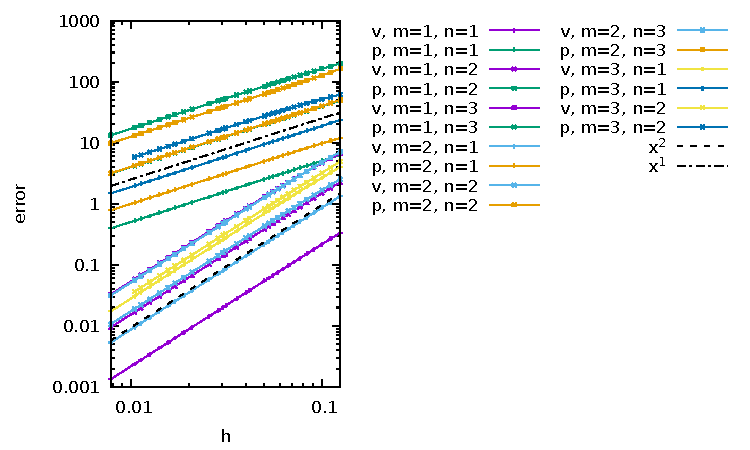
\includegraphics[width=12cm]{python_codes/fieldstone_32/results/errors}\\
{\captionfont Discrerization errors for velocity and pressure for various $(m,n)$ values.}
\end{center}
Note that the assembly proces in the code is somewhat naive and therefore limits
the maximum resolution to about $128\times 128$ elements.

\begin{center}
\includegraphics[width=10cm]{python_codes/fieldstone_32/results/vel_2x1}\\
{\captionfont Velocity arrows for $(m,n)=(2,1)$}
\end{center}
